\let\negmedspace\undefined
\let\negthickspace\undefined
\documentclass[journal]{IEEEtran}
\usepackage[a5paper, margin=10mm, onecolumn]{geometry}
%\usepackage{lmodern} % Ensure lmodern is loaded for pdflatex
\usepackage{tfrupee} % Include tfrupee package

\setlength{\headheight}{1cm} % Set the height of the header box
\setlength{\headsep}{0mm}     % Set the distance between the header box and the top of the text

\usepackage{gvv-book}
\usepackage{gvv}
\usepackage{cite}
\usepackage{amsmath,amssymb,amsfonts,amsthm}
\usepackage{algorithmic}
\usepackage{graphicx}
\usepackage{textcomp}
\usepackage{xcolor}
\usepackage{txfonts}
\usepackage{listings}
\usepackage{enumitem}
\usepackage{mathtools}
\usepackage{gensymb}
\usepackage{comment}
\usepackage[breaklinks=true]{hyperref}
\usepackage{tkz-euclide} 
\usepackage{listings}
\usepackage{gvv}                                        
\def\inputGnumericTable{}                                 
\usepackage[latin1]{inputenc}                                
\usepackage{color}                                            
\usepackage{array}                                            
\usepackage{longtable}                                       
\usepackage{calc}                                             
\usepackage{multirow}                                         
\usepackage{hhline}                                           
\usepackage{ifthen}                                           
\usepackage{lscape}
\begin{document}

\bibliographystyle{IEEEtran}

\title{5.8.17}
\author{EE25BTECH11019 - Darji Vivek M.}
{\let\newpage\relax\maketitle}

\renewcommand{\thefigure}{\theenumi}
\renewcommand{\thetable}{\theenumi}
\setlength{\intextsep}{10pt}
\numberwithin{figure}{enumi}
\renewcommand{\thetable}{\theenumi}

\textbf{Question}:\\
A fraction becomes $\frac{9}{11}$ if $2$ is added to both the numerator and the denominator. If $3$ is added to both the numerator and the denominator, it becomes $\frac{5}{6}$. Find the fraction.\\[4pt]

\solution \\[-2mm]

\textbf{Matrix Method:}\\
Let the numerator be $n$ and the denominator be $d$. From the conditions we get
\begin{align}
\frac{n+2}{d+2} &= \frac{9}{11} \quad\Longrightarrow\quad 11(n+2)=9(d+2) \;\Longrightarrow\; 11n-9d=-4,\\
\frac{n+3}{d+3} &= \frac{5}{6}  \quad\Longrightarrow\quad 6(n+3)=5(d+3) \;\Longrightarrow\; 6n-5d=-3.
\end{align}

In matrix form:
\begin{align}
\myvec{11 & -9\\[2pt] 6 & -5}\myvec{n\\[2pt] d}=\myvec{-4\\[2pt]-3}.
\end{align}

Solve by row-reduction (augmented matrix). In the same \texttt{\textbackslash augvec} format you provided:
\[
\resizebox{1\textwidth}{!}{$
\augvec{2}{3}{11 & -9 & -4\\ 6 & -5 & -3}
\xrightarrow{R_1 \gets \frac{1}{11}R_1,\ R_2 \gets R_2 - 6R_1}
\augvec{2}{3}{1 & -\frac{9}{11} & -\frac{4}{11}\\[2pt] 0 & -\frac{1}{11} & -\frac{9}{11}}
\xrightarrow{R_2 \gets -11R_2,\ R_1 \gets R_1 + \frac{9}{11}R_2}
\augvec{2}{3}{1 & 0 & 7\\[2pt] 0 & 1 & 9}
$}
\]

Thus
\begin{align}
n &= 7, & d &= 9.
\end{align}

Therefore the fraction is \(\boxed{\frac{7}{9}}\).\\[4pt]

\textbf{Check:}\quad \(\frac{7+2}{9+2}=\frac{9}{11},\quad \frac{7+3}{9+3}=\frac{10}{12}=\frac{5}{6}.\)

 \begin{figure}[H]
     \centering
     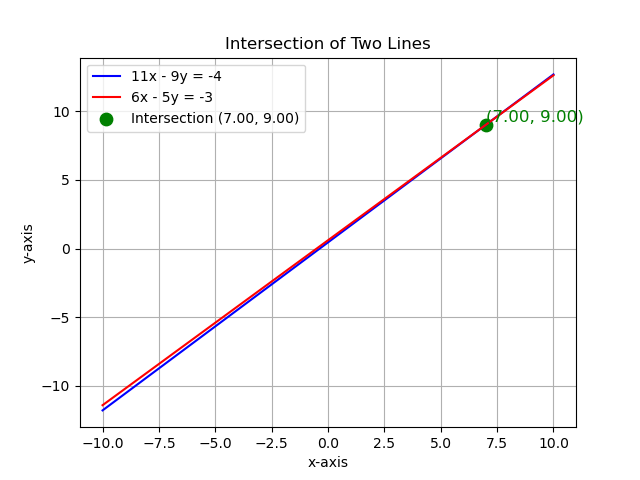
\includegraphics[width=0.8\columnwidth]{figs/12.png}
     \label{fig:1}
 \end{figure}

\end{document}